This section will give an introduction to the available test system, including structure and components overview.  

\section{System overview}
\label{system_overview}
To develop and test different control methods for a water distribution system a test setup is required.
Such a setup is available at Aalborg university which is based on a real water distribution system, though as a 1:20 downscaled version.

%picture of test system
\begin{figure}[H]
\centering
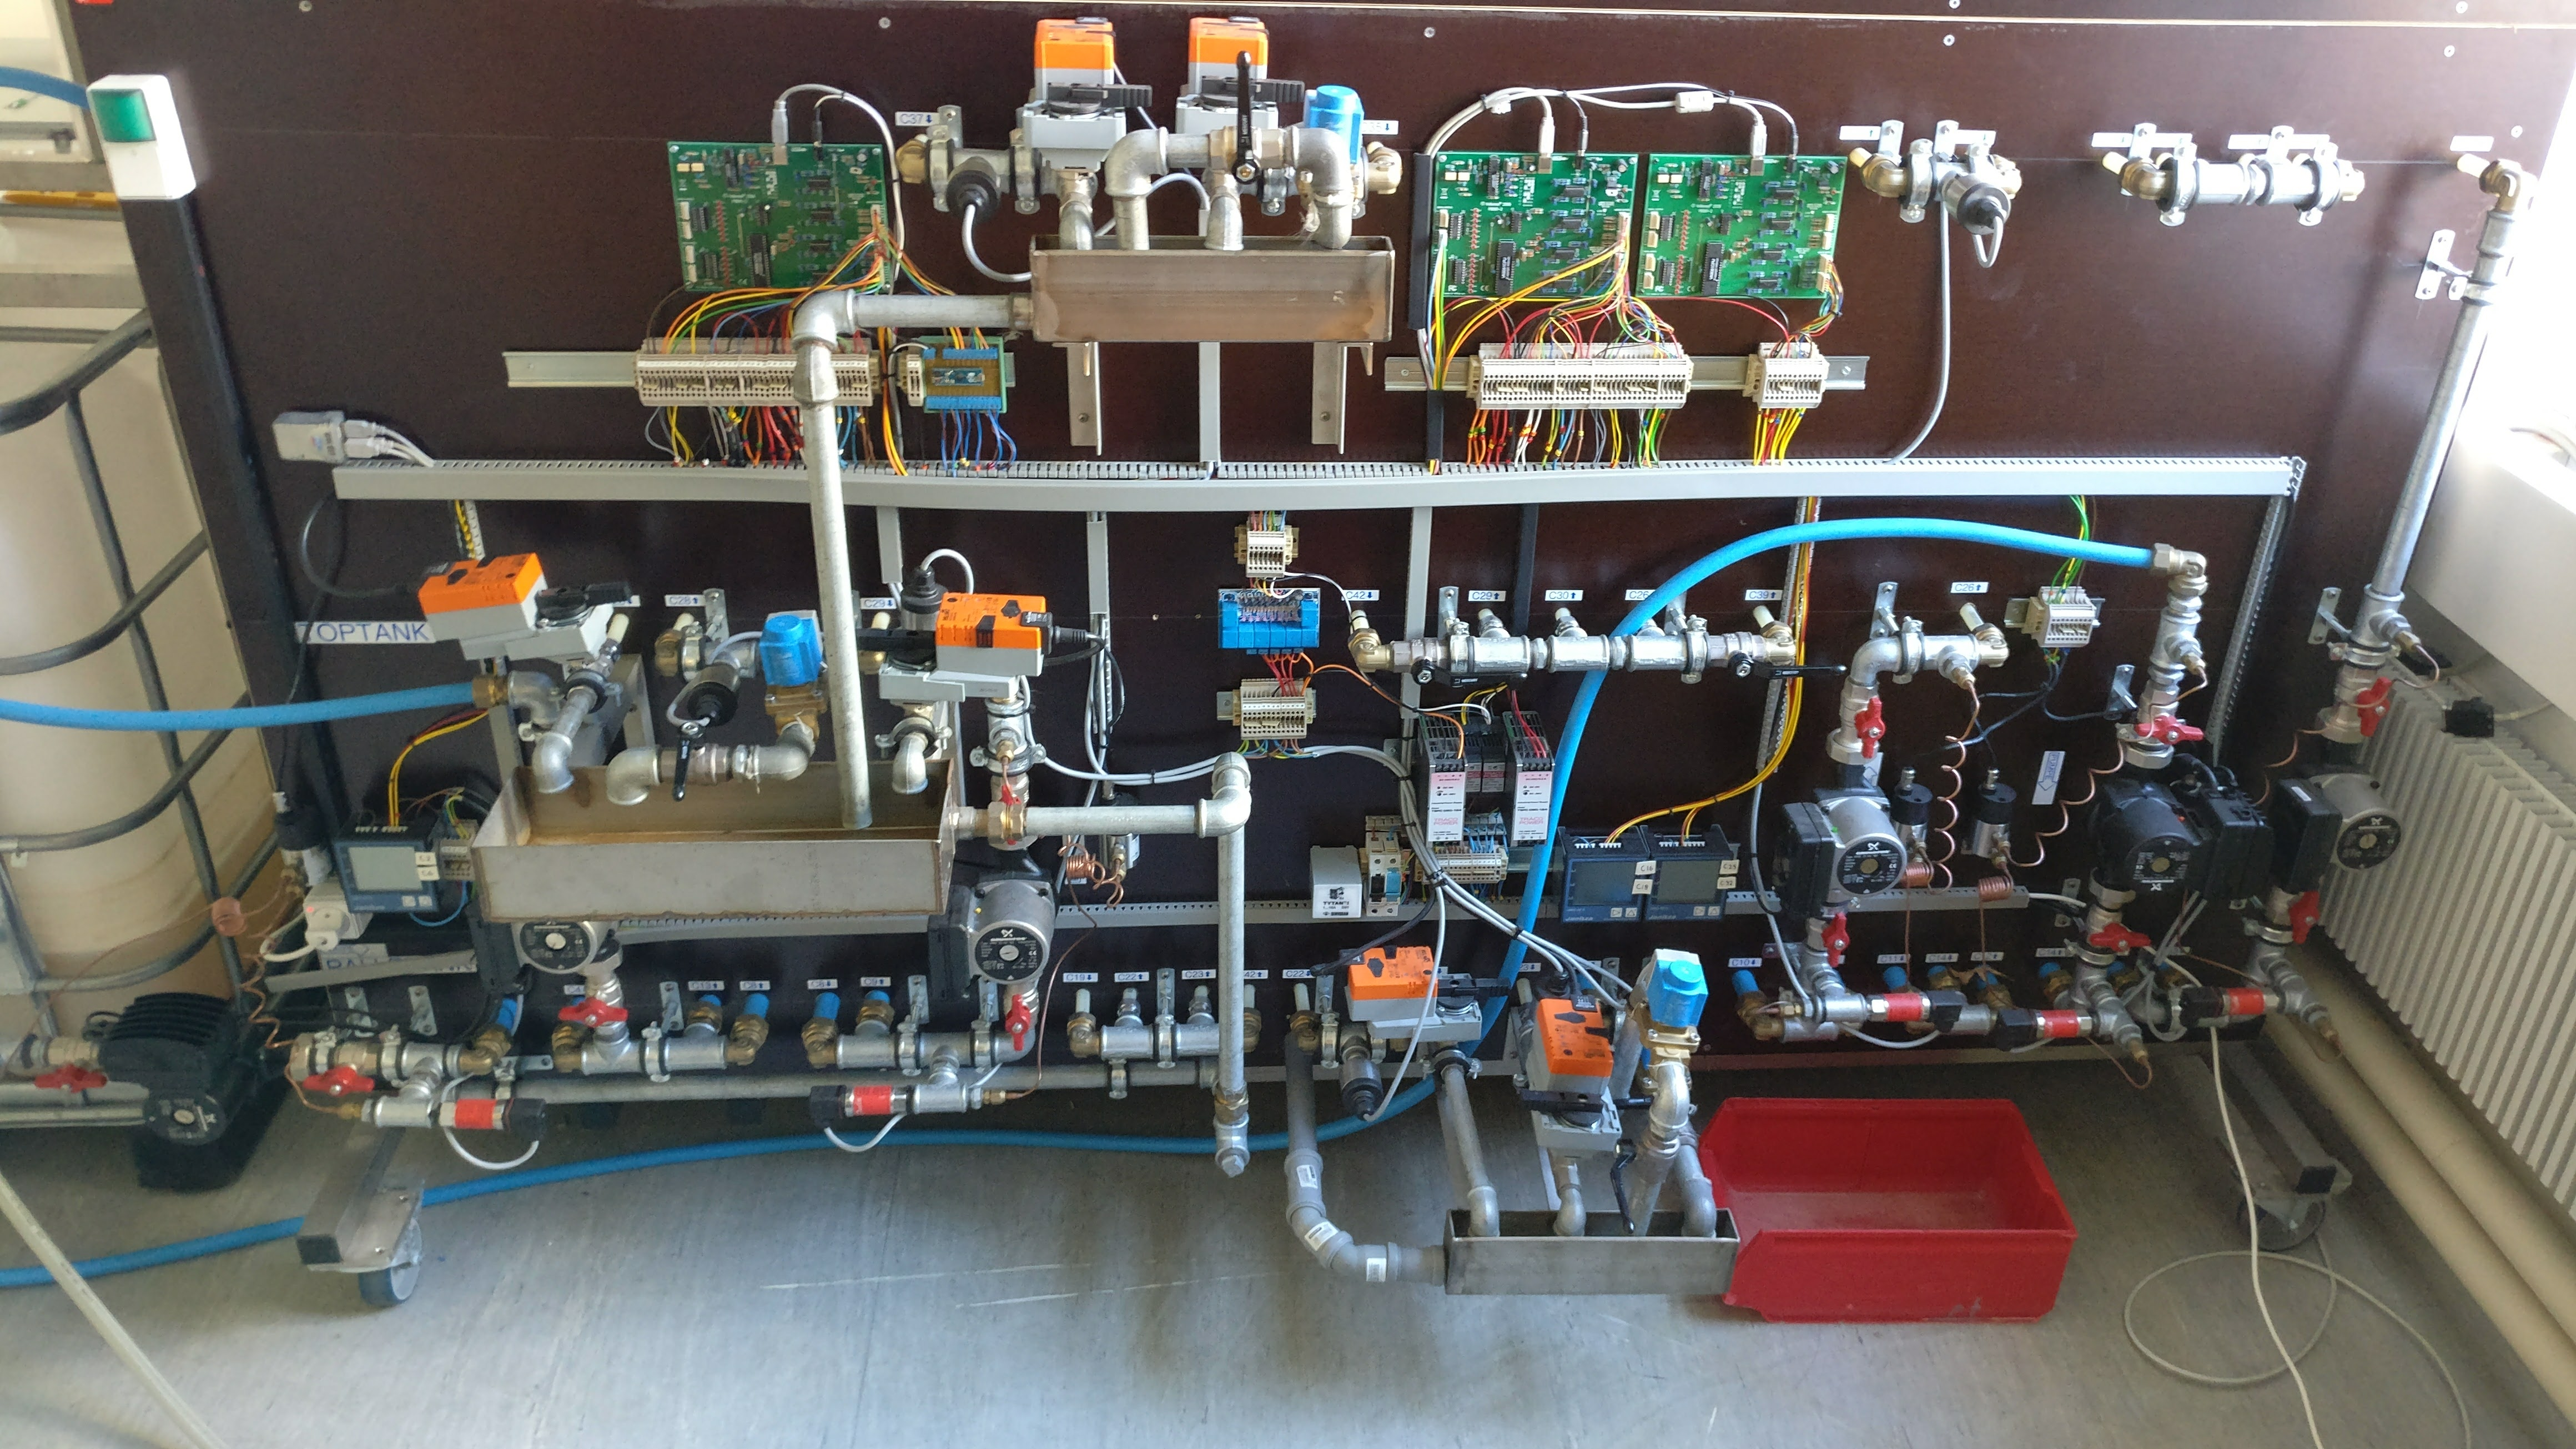
\includegraphics[width=0.85\textwidth]{report/pictures/test_system_wide}
\caption{The available test setup used to represent a real water distribution system.}
\label{fig:test_setup}
\end{figure}


The test setup represents a real system, thus the same structure concerning piping, levelling and all the other components. To achieve different elevation levels between system parts, the setup is mounted on a wall. This also allows for a quick overview of the complete setup and eases access to the components. As the system is used for various test scenarios other equipment are also present in the test setup shown in \figref{fig:test_setup}, enabling the test system to mimic a variety of different system types and scenarios. A diagram representing the part of the test setup that will be used in this project is shown in \figref{fig:sys_model_overview}. 

%tikz of our system
\begin{figure}[H]
\centering
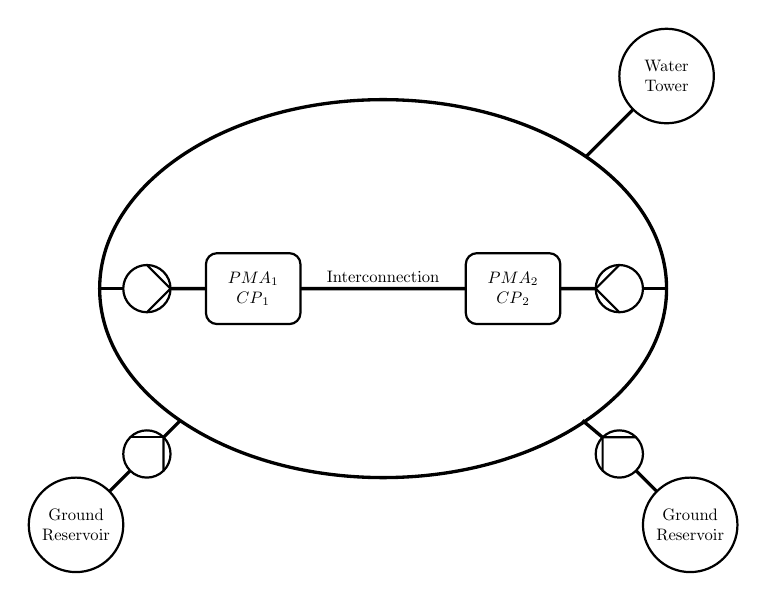
\begin{tikzpicture}[scale=0.6,transform shape]
\tikzstyle{box} = [draw,thick,rounded corners, minimum height=15mm, minimum width=20mm, align=center, text centered]
%Main Ring
\draw[very thick] (7,5.5) ellipse (6 and 4);
%Pump
\draw[thick,transform shape] (2,5.5) circle (0.5);
\draw[thick,transform shape] (2.5,5.5) -- (2,6);
\draw[thick,transform shape] (2.5,5.5) -- (2,5);
%Pump
\begin{scope} [rotate around={180:(12,5.5)}]
\draw[thick,transform shape] (12,5.5) circle (0.5);
\draw[thick,transform shape] (12.5,5.5) -- (12,6);
\draw[thick,transform shape] (12.5,5.5) -- (12,5);
\end{scope}
%Pump
\begin{scope} [rotate around={135:(12,2)}]
\draw[thick,transform shape] (12,2) circle (0.5);
\draw[thick,transform shape] (12.5,2) -- (12,2.5);
\draw[thick,transform shape] (12.5,2) -- (12,1.5);
\end{scope}
%Pump
\begin{scope} [rotate around={45:(2,2)}]
\draw[thick,transform shape] (2,2) circle (0.5);
\draw[thick,transform shape] (2.5,2) -- (2,2.5);
\draw[thick,transform shape] (2.5,2) -- (2,1.5);
\end{scope}
%Reservoirs
\node[thick,draw,circle,minimum width=20mm,align=center] (R1) at (0.5,0.5) {Ground \\ Reservoir};
\node[thick,draw,circle,minimum width=20mm,align=center] (ER1) at (13,10) {Water \\ Tower};
\node[thick,draw,circle,minimum width=20mm,align=center] (R2) at (13.5,0.5) {Ground \\ Reservoir};
%PMA and interconnection
\node[box] (PMA1) at (4.25,5.5) {$\text{PMA}_1$ \\ $\text{CP}_1$};
\node[box] (PMA2) at (9.75,5.5) {$\text{PMA}_2$ \\ $\text{CP}_2$};
\draw[very thick](PMA1) -- (PMA2);
\node[align=center] (PMAc) at (7,5.75) {Interconnection};
%Connections
\draw[very thick](1.2,1.2) -- (1.65,1.65);
\draw[very thick](2.34,2.34) -- (2.71,2.71);
\draw[very thick](12.8,1.2) -- (12.36,1.64);
\draw[very thick](11.66,2.34) -- (11.22,2.71);
\draw[very thick](13,5.5) -- (12.5,5.5);
\draw[very thick](11.5,5.5) -- (PMA2);
\draw[very thick](1,5.5) -- (1.5,5.5);
\draw[very thick](2.5,5.5) -- (PMA1);
\draw[very thick](12.28,9.28) -- (11.29,8.29);
\end{tikzpicture} 
\caption{Overview of the reduced system that fulfills the scenario of this project.}
\label{fig:sys_model_overview}
\end{figure}
\todo{Should we consider changing the name "elevated reservoir" to "water tower". We have uesed the word water tower in the introduction}

The system consists of different parts, the main part being a water reservoir placed on ground level, used to supply the system. Two pumps are connected to the reservoir and they supply water to the main water ring formed around the consumers. 
Another water reservoir is connected to the water ring by a dedicated pump. This reservoir is elevated and can, when filled, be used to pressurize the system. 
From the water ring two PMA's are connected via their own pump. In each PMA a measuring point is placed and the pressure at this point shall be kept. Furthermore two consumers are placed in each PMAs.         
	
\begin{figure}
	\centering
	\begin{minipage}[b]{0.6\textwidth}
		\centering
		\tikzset{pressure/.style={draw, circle, inner sep=0pt, text width=4mm, align=center}}
\tikzset{difpres/.style={draw, circle, inner sep=0pt, text width=5mm, align=center}}
\tikzset{connect/.style={draw,circle, inner sep=0pt, text width=2mm, align=center,fill=black}}
\tikzset{evalve/.style={draw, circle, inner sep=0pt, text width=3mm, align=center}}
\begin{tikzpicture} [scale=0.7,transform shape]
%Pump
\begin{scope} [rotate around={90:(0,1)}, shift={(0,1)}]
\draw[transform shape] (0,0) circle (0.5);
\draw[transform shape] (0.5,0) -- (0,0.5);
\draw[transform shape] (0.5,0) -- (0,-0.5);
\end{scope}

%man-valve
\node(n1) at (0.25,3.5) {};
\node(n2) at (-0.25,3.5) {};
\node(n3) at (0.25,2.5) {};
\node(n4) at (-0.25,2.5) {};
\node(n5) at (0,3) {};
\node(n6) at (-0.5,3.25) {};
\node(n7) at (-0.5,2.75) {};
\draw(n1.center)--(n2.center)--(n3.center)--(n4.center)--(n1.center)--(n2.center);
\draw(n5.center)-|(n6.center)--(n7.center);

%elec-valve
\node(n1) at (4.25,3.5) {};
\node(n2) at (3.75,3.5) {};
\node(n3) at (4.25,2.5) {};
\node(n4) at (3.75,2.5) {};
\node(n5) at (4,3) {};
\node[evalve] (n6) at (3.5,3) {};
\draw(n1.center)--(n2.center)--(n3.center)--(n4.center)--(n1.center)--(n2.center);
\draw(n5.center)--(n6);

%man-valve
\node(n1) at (0.25,-0.5) {};
\node(n2) at (-0.25,-0.5) {};
\node(n3) at (0.25,-1.5) {};
\node(n4) at (-0.25,-1.5) {};
\node(n5) at (0,-1) {};
\node(n6) at (-0.5,-0.75) {};
\node(n7) at (-0.5,-1.25) {};
\draw(n1.center)--(n2.center)--(n3.center)--(n4.center)--(n1.center)--(n2.center);
\draw(n5.center)-|(n6.center)--(n7.center);

%man-valve
%\draw[very thick](-0.25,-1) -- (0.25,-1) -- (-0.25,-2) -- (0.25,-2) -- (-0.25,-1) -- (0.25,-1);
%\draw[very thick](0,-1.5) -- (-0.5,-1.5);
%\draw[very thick](-0.5,-1.25) -- (-0.5,-1.75);

%GND
\draw(-0.3,-2.5)--(0.3,-2.5);
\draw(-0.15,-2.6)--(0.15,-2.6);

%GND
\draw(3.7,1.5)--(4.3,1.5);
\draw(3.85,1.4)--(4.15,1.4);

%pipe
%right arcs
\draw (2.5,5.5) arc (90:-90:0.05);
\draw (2.5,5.3) arc (90:-90:0.05);
\draw (2.5,5.1) arc (90:-90:0.05);
%left arcs
\draw (1,5.4) arc (90:270:0.05);
\draw (1,5.2) arc (90:270:0.05);
\draw (1,5) arc (90:270:0.05);
%lines
\draw(1,5.5) -- (2.5,5.5);
\draw(1,5.4) -- (2.5,5.4);
\draw(1,5.3) -- (2.5,5.3);
\draw(1,5.2) -- (2.5,5.2);
\draw(1,5.1) -- (2.5,5.1);
\draw(1,5) -- (2.5,5);
\draw[rounded corners](1,4.9) -- (2.65,4.9) -- (2.65,5.5) -- (3.4,5.5);
%pipe name
%\node at (2,4) {$\text{C}_1$};

%pressure sensor
\node[connect] (PD1) at (3.5,5.5) {};
\node(P1) at ($(PD1)+(0,1)$) [pressure] {P};
\draw(PD1) -- (P1);

%differential pressure sensor
\node[connect] (CDP1) at (0,4) {};
\node[connect] (CDP2) at (0,-2) {};
\node[difpres] (DP1) at (-1.5,0.5) {DP};
\draw(CDP1) -| (DP1)  |- (CDP2);

%Connections
\draw(0,1.5) -- (0,2.5);
\draw(0,0.5) -- (0,-0.5);
\draw(0,-1.5) -- (0,-2.5);
\draw[rounded corners](0,3.5)--(0,5.5)--(1,5.5);
\draw[rounded corners](3,5.5)--(4,5.5)--(4,3.5);
\draw(4,2.5) -- (4,1.5);

\end{tikzpicture}

     
		\caption{Basic water distribution network.}
		\label{fig:Basic_example_sys}
	\end{minipage}
	\hspace{15pt}
	\begin{minipage}[b]{0.3\textwidth}
		\begin{tabular}{|c|c|} \hline
  			\bfseries Symbol 	 					&   \bfseries Name 					\\ \hline
			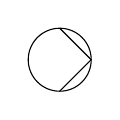
\begin{tikzpicture}[scale=0.8,transform shape]
%Pump
\draw (0,0) circle (0.5);
\draw (0.5,0) -- (0,0.5);
\draw (0.5,0) -- (0,-0.5);
\addvmargin{4mm}
\end{tikzpicture}

     		  	&	Pump							\\ \hline
			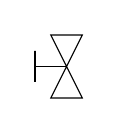
\begin{tikzpicture}[scale=0.8,transform shape]
%man-valve
\node(n1) at (0.25,2) {};
\node(n2) at (-0.25,2) {};
\node(n3) at (0.25,1) {};
\node(n4) at (-0.25,1) {};
\node(n5) at (0,1.5) {};
\node(n6) at (-0.5,1.75) {};
\node(n7) at (-0.5,1.25) {};
\draw(n1.center)--(n2.center)--(n3.center)--(n4.center)--(n1.center)--(n2.center);
\draw(n5.center)-|(n6.center)--(n7.center);
\addvmargin{4mm}
\end{tikzpicture}

     	&	Manual valve					\\ \hline
			\tikzset{evalve/.style={draw, circle, inner sep=0pt, text width=3mm, align=center}}
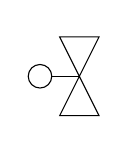
\begin{tikzpicture}
%elec-valve
\node(n1) at (4.25,2) {};
\node(n2) at (3.75,2) {};
\node(n3) at (4.25,1) {};
\node(n4) at (3.75,1) {};
\node(n5) at (4,1.5) {};
\node(n6) at (3.5,1.5) [evalve] {};
\draw(n1.center)--(n2.center)--(n3.center)--(n4.center)--(n1.center)--(n2.center);
\draw(n5.center)--(n6);
\addvmargin{4mm}
\end{tikzpicture}

     		&	Electronic valve				\\ \hline
			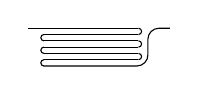
\begin{tikzpicture}[scale=0.8,transform shape]
%pipe
%right arcs
\draw (2.5,3.5) arc (90:-90:0.05);
\draw (2.5,3.3) arc (90:-90:0.05);
\draw (2.5,3.1) arc (90:-90:0.05);
%left arcs
\draw (1,3.4) arc (90:270:0.05);
\draw (1,3.2) arc (90:270:0.05);
\draw (1,3) arc (90:270:0.05);
%lines
\draw(0.75,3.5) -- (2.5,3.5);
\draw(1,3.4) -- (2.5,3.4);
\draw(1,3.3) -- (2.5,3.3);
\draw(1,3.2) -- (2.5,3.2);
\draw(1,3.1) -- (2.5,3.1);
\draw(1,3) -- (2.5,3);
\draw[rounded corners](1,2.9) -- (2.65,2.9) -- (2.65,3.5) -- (3,3.5);
\addvmargin{4mm}
\end{tikzpicture}

     		  	&	Pipe segment					\\ \hline
			\tikzset{pressure/.style={draw, circle, inner sep=0pt, text width=4mm, align=center}}
\tikzset{difpres/.style={draw, circle, inner sep=0pt, text width=5mm, align=center}}
\tikzset{connect/.style={draw,circle, inner sep=0pt, text width=2mm, align=center,fill=black}}
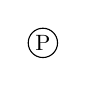
\begin{tikzpicture}[scale=0.8,transform shape]
%pressure sensor
\node(P1) at (0,0) [pressure] {P};
\addvmargin{4mm}
\end{tikzpicture}

     &	Pressure sensor					\\ \hline
			\tikzset{pressure/.style={draw, circle, inner sep=0pt, text width=4mm, align=center}}
\tikzset{difpres/.style={draw, circle, inner sep=0pt, text width=5mm, align=center}}
\tikzset{connect/.style={draw,circle, inner sep=0pt, text width=2mm, align=center,fill=black}}

\begin{tikzpicture}[scale=0.8,transform shape]
%differential pressure sensor
\node(DP1) at (-2,0) [difpres] {DP};
\addvmargin{4mm}
\end{tikzpicture}

     	&	Differential pressure sensor	\\ \hline
			\begin{tikzpicture}[scale=0.8,transform shape]
%GND
\draw(-0.3,-2.5)--(0.3,-2.5);
\draw(-0.15,-2.6)--(0.15,-2.6);
\draw(0,-2.5)--(0,-2);
\addvmargin{4mm}
\end{tikzpicture}

     		  	&	Gnd								\\ \hline
		\end{tabular}
		\captionof{table}{Symbol and name for component in the water network.}	
		\label{tab:sys_comp_overview}
	\end{minipage}
\end{figure}
%\end{minipage}